\documentclass{article}

\usepackage[utf8]{inputenc}
\usepackage[letterpaper,top=2cm,bottom=2cm,left=3cm,right=3cm,marginparwidth=1.75cm]{geometry}
\usepackage[english]{babel}
\usepackage{graphicx}
\usepackage[colorlinks=false, allcolors=black, hidelinks=true]{hyperref}
\usepackage{biblatex}
\addbibresource{IVI.bib}

\title{Interactive Visualizations (IVI) Bericht}
\author{Nicola Rohner}
\date{SE FE 2023}

\begin{document}

\maketitle

\begin{center}
\textbf{Repository:} \url{https://github.com/nicolarohner1337/ivi}
\end{center}

\begin{abstract}
In diesem Bericht werden die Lernergebnisse des Moduls IVI zusammengefasst.\\
Für alle ausser LE1 wurden folgende Daten verwendet: \newline
GroupLens Research hat Bewertungsdatensätze von der MovieLens-Website \url{https://movielens.org} gesammelt und zur Verfügung gestellt.
Die Datensätze wurden über verschiedene Zeiträume hinweg gesammelt, abhängig von der Größe des Satzes. Das ZIP findet man unter folgendem Link: \url{https://files.grouplens.org/datasets/movielens/ml-latest.zip}
Die Daten umfassen 27.000.000 Bewertungen und 1.100.000 Tag-Anwendungen für 58.000 Filme von 280.000 Nutzern. Beinhaltet Tag-Genom-Daten mit 14 Millionen Relevanz-Scores für 1.100 Tags.\\
\noindent\\
Die Visualisierungen in diesem Bericht wurden alle selbst erstellt. 
Der Datensatz wurde bereits für die Challenge CDS1 genutzt und für die Erarbeitung von GDV.
\end{abstract}

\tableofcontents

\newpage

\section{LE1: Performance}
In Zeiten von Big Data ist es wichtig, dass Visualisierungen schnell und performant sind. In diesem LE wird untersucht, wie sich die Performance von Visualisierungen auf verschiedene Arten beeinflussen lässt.


\subsection{WebGL}
WebGL ist eine leistungsstarke Technologie, die Berechnungen beschleunigt. Allerdings gibt es einige Einschränkungen.
WebGL benötigt eine GPU (Grafikkarte), die nicht immer in allen Browsern verfügbar ist.
Mit WebGL gerenderte Daten werden als Pixelraster gezeichnet, was in einigen Fällen zu verpixelten oder unscharfen Bildern führen kann.
Browser begrenzen die Anzahl der WebGL Kontexte, auf die ein bestimmtes Webdokument zugreifen kann, was die Darstellung von WebGL-Visualisierungen einschränken kann.
Browser setzen Grenzen für die Höhe und Breite von Visualisierungen, die WebGL verwenden, was bei extrem großen Plots zu Problemen führen kann.\cite{plotly_webgl_nodate}
%hard break
\newline
\newline
Um die Performance Unterschiede zu untersuchen habe ich eine Visualisierung erstellt, welche 100000 zufällige Punkte in einem 2D Koordinatensystem darstellt.
Einmal wurde die Visualisierung mit dem Modus SVG und einmal mit WebGL gerendert. Was bereits qualitativ auffällt ist, dass die WebGL Visualisierung deutlich schneller angezeigt wird im Chrome Browser.

%enter image here
\begin{figure}[!h]
\centering
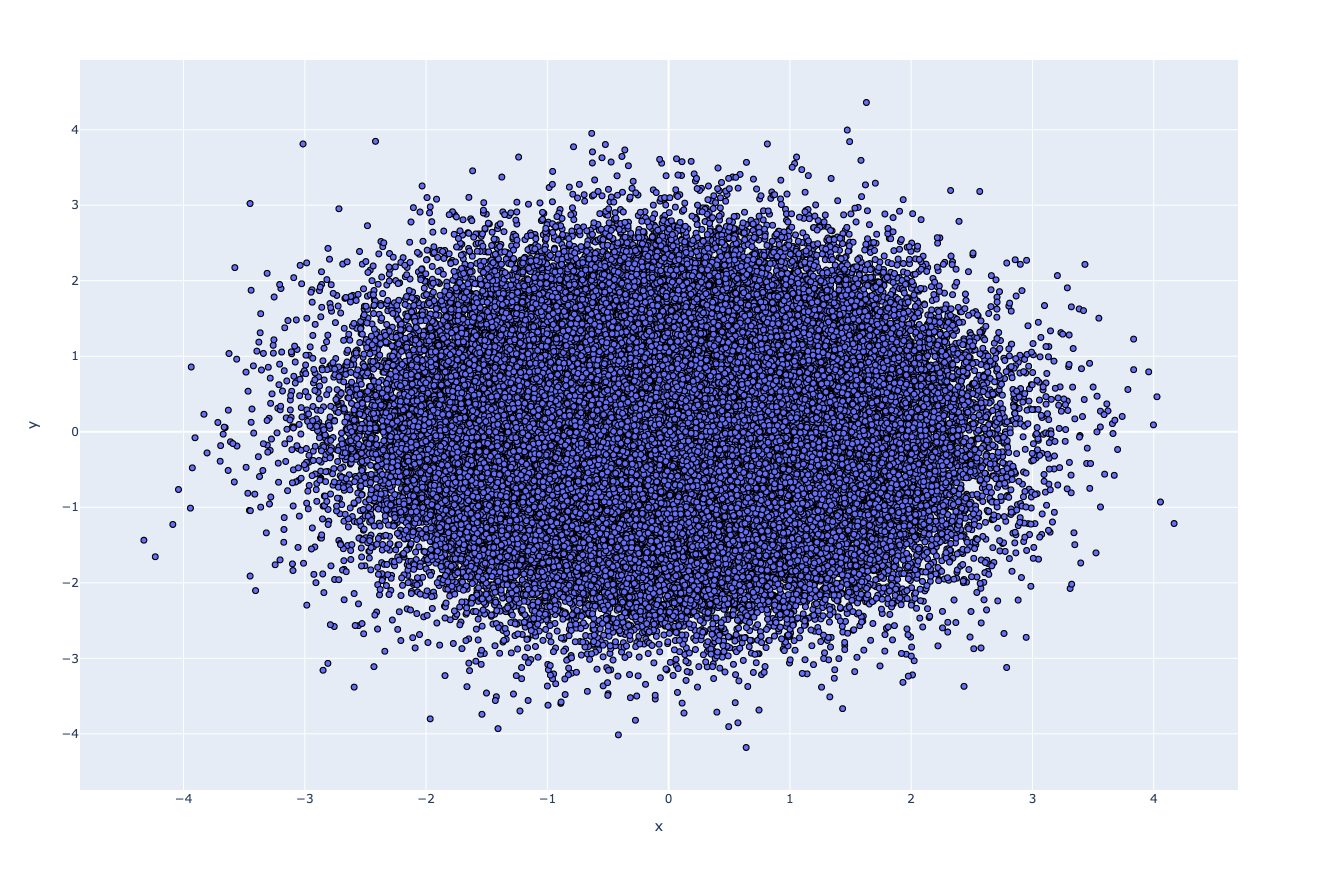
\includegraphics[width=0.3\textwidth]{img/random_dots.png}


\caption{\label{fig: LE1 Random Dots plot}Random dots}
\end{figure}

\noindent
Die Chrome Entwickler Tools verfügen über ein Performance Profiler Tool, welches die Performance einer Webseite analysieren kann. Es unterteilt die Laufzeitleistung in das RAIL-Modell\cite{noauthor_measure_nodate}: Response, Animation, Idle und Load.
Im Kontext zur Visualisierung betrachte man die Scripting, Rendering und Painting Kategorien.\cite{kayce_basques_analyze_nodate}

%enter table here
\begin{table}[!h]
\centering
\begin{tabular}{|l|l|l|l|}
\hline
\textbf{Kategorie} & \textbf{SVG} & \textbf{WebGL} & \textbf{\%$\Delta$} \\
\hline
Scripting & 3778ms & 651ms & -580\% \\
\hline
Rendering & 2026ms & 14ms & -1447\% \\
\hline
Painting & 197ms & 2ms & -985\% \\
\hline
\end{tabular}
\caption{\label{tab: LE1 Performance}Performance Unterschiede}
\end{table}

\noindent
Zu beobachten ist ein signifikanter Unterschied in den Rendering und Painting Zeiten der beiden Visualisietungen. Auch die subjektive Wahrnehmung der Performance ist deutlich besser bei der WebGL Visualisierung.
Auch die Tradeoffs zwischen Performance und Qualität sind deutlich zu erkennen. Die SVG Visualisierung ist deutlich schärfer und die Punkte sind deutlich besser zu erkennen.
\begin{figure}[!h]
\centering
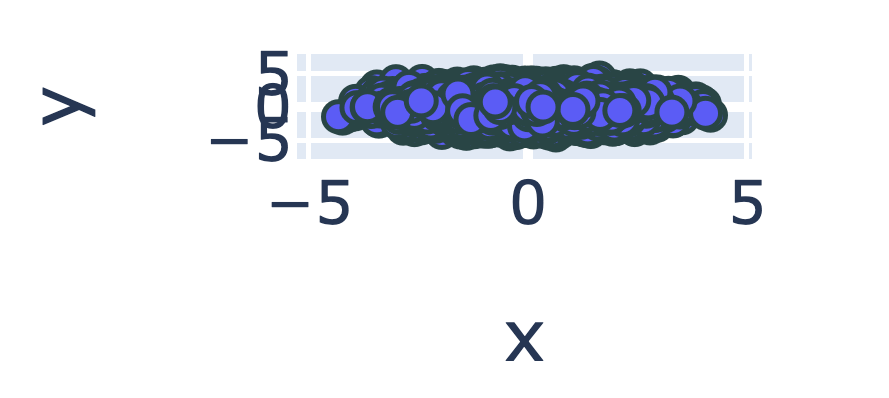
\includegraphics[width=0.4\textwidth]{img/svg_quality.png}
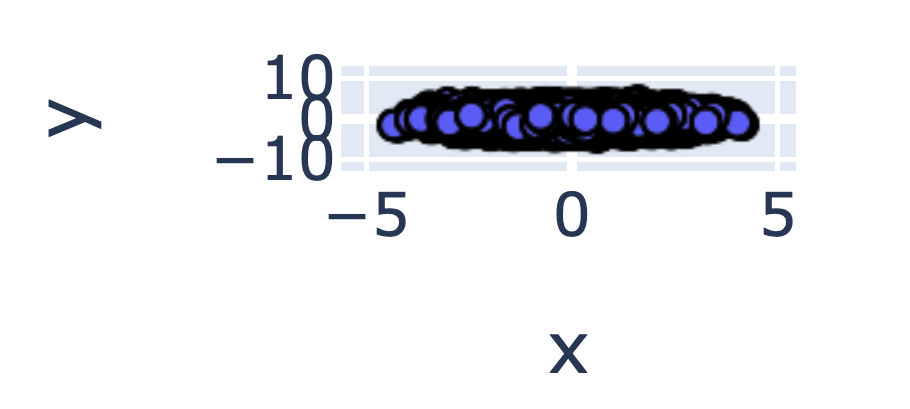
\includegraphics[width=0.4\textwidth]{img/webgl_quality.png}
\setlength{\belowcaptionskip}{-10pt}
\caption{\label{fig: LE1 Qualität Unterschiede} Qualität Unterschiede links SVG, rechts WebGL}
\end{figure}
\newpage

\subsection{Layering}
Datashader ist ein Grafik-Pipeline-System zur schnellen und flexiblen Erstellung aussagekräftiger Darstellungen grosser Datensätze. Datashader unterteilt die Erstellung von Bildern in eine Reihe expliziter Schritte, die es ermöglichen, Berechnungen an Zwischendarstellungen vorzunehmen.\cite{wong_abstract_2013}
\newline
Wir visualisieren hier die räumliche Verteilung der Taxifahrten in New York City. 
Die Daten werden von Plotly zu Verfügung gestellt und sind unter folgendem Link zu finden: \url{https://raw.githubusercontent.com/plotly/datasets/master/uber-rides-data1.csv}

\begin{table}[!h]
\centering
\begin{tabular}{|l|l|}
\hline
\textbf{Date/Time} & \textbf{The date and time of the Uber pickup} \\
\hline
\textbf{Lat} & \textbf{The latitude of the Uber pickup} \\
\hline
\textbf{Lon} & \textbf{The longitude of the Uber pickup} \\
\hline
\end{tabular}
\caption{\label{tab: LE1 Newyork Taxi Data} Newyork Uber Data}
\end{table}



%enter image here
\begin{figure}[!h]
\centering
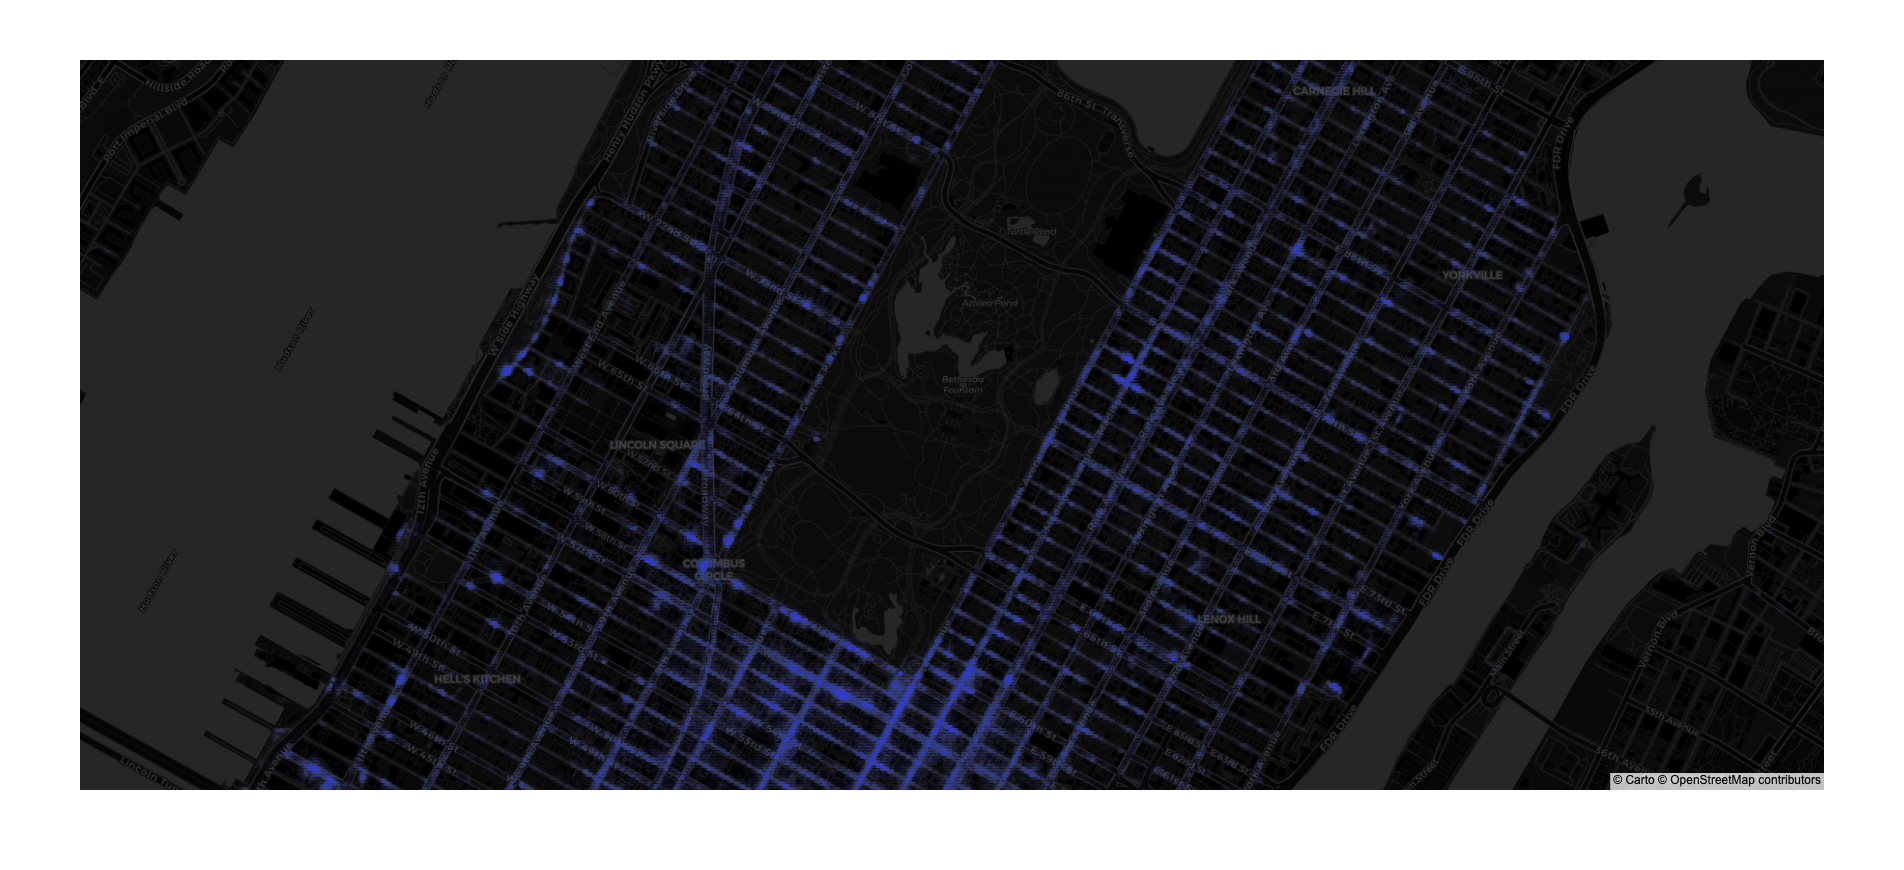
\includegraphics[width=0.4\textwidth]{img/newyork_plotly.png}
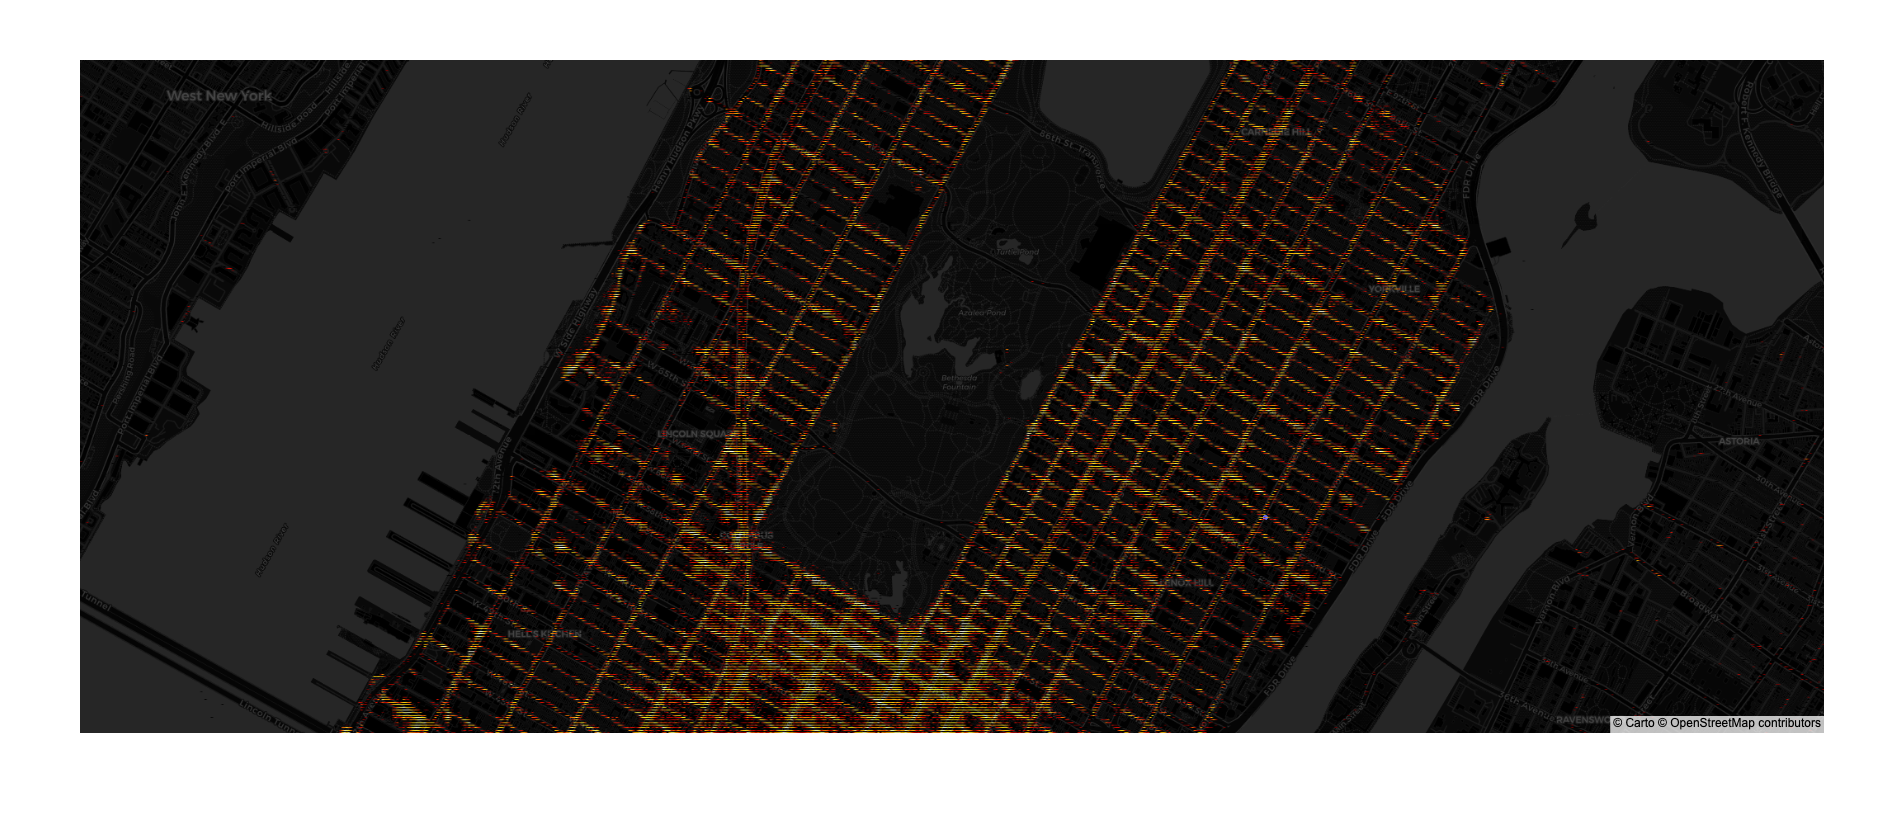
\includegraphics[height=0.18\textwidth]{img/newyork_datashader.png}
\caption{\label{fig: LE1 Plotly vs Datashader} Taxifahrten in Newyork (Plotly links, Datashader Layer rechts)}
\end{figure}
\noindent
Zu beobachten ist das die unprozessierten Daten mit Plotly zwar schöner dargestellt werden. Aber viel länger brauchen um angezeigt zu werden. Die Datashader Visualisierung ist deutlich schneller und die Daten werden deutlich besser dargestellt.
Diese Beobachtungen wiederspiegeln sich auch in den Performance Daten. Zwar wird nur die Scripting Zeit signifikant verkürzt.


%enter table here
\begin{table}[!h]
    \centering
    \begin{tabular}{|l|l|l|l|}
    \hline
    \textbf{Kategorie} & \textbf{Plotly} & \textbf{Datashader Layer} & \textbf{\%$\Delta$} \\
    \hline
    Scripting & 1241ms & 492ms & -39\% \\
    \hline
    Rendering & 6ms & 6ms & $\pm$0\% \\
    \hline
    Painting & 12ms & 12ms & $\pm$0\% \\
    \hline
    \end{tabular}
    \caption{\label{tab: LE1 Performance}Performance Unterschiede}
\end{table}
\noindent
Spannender bei diesem Fall sind die Unteschiede des genutzen Speichers. Wenn wir den JavaScript Heap betrachten sehen wir einen signifikanten Unterschied\cite{noauthor_memory_2023}.
Plotly braucht fast 130MB um die Daten zu visualisieren, der Datashader Layer braucht nur 23MB.

%enter image here
\begin{figure}[!h]
\centering
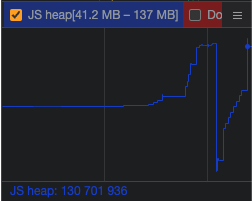
\includegraphics[width=0.2\textwidth]{img/js_heap_plotly.png}
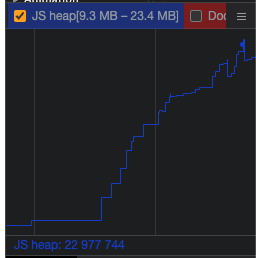
\includegraphics[height=0.158\textwidth]{img/js_heap_datashader.png}
\caption{\label{fig: LE1 Datashader Memory} Memory Heap Plotly vs. Datashader Layer}
\end{figure}
\noindent
Einen ähnlichen Ansatz verfolgen auch Framworks wie Deck.gl. Diese Frameworks sind jedoch auf WebGL basiert und können somit nur auf Browsern mit WebGL Unterstützung verwendet werden.
Sie prozessieren für verschiedene Ansichte voragregierte Layers und können so sehr schnell und performant visualisieren.\cite{deckgl_home_nodate}

\newpage
\printbibliography


\end{document}